\section{E --- The Lakes (Codeforces)}

\subsection*{Código}
\lstinputlisting{E_TheLakes/Main.java}

\subsection*{Comprovante de aceite}
\begin{center}
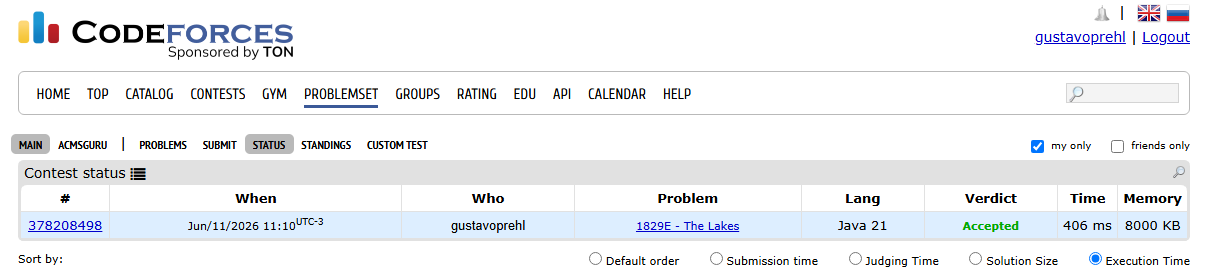
\includegraphics[width=0.85\textwidth]{Accepts/E_TheLakes.png}
\end{center}

\subsection*{Justificativa}

\textbf{Estratégia:} componentes conexas em grade (BFS), com leitura rápida e
fila explícita por questões de desempenho.

\textbf{Modelagem:} cada célula com \texttt{a[i][j] > 0} é um vértice de um
grafo implícito, com arestas para os vizinhos ortogonais (cima, baixo,
esquerda, direita) que também tenham valor $> 0$. Um ``lago'' é exatamente
uma componente conexa desse grafo, e seu ``volume'' é a soma dos valores dos
vértices da componente. O problema pede o maior volume entre todas as
componentes --- ou 0 se não existir nenhuma célula com valor $> 0$.

\textbf{Algoritmo:} percorre-se cada célula da grade; se ainda não foi
visitada e tem valor $> 0$, executa-se uma BFS a partir dela, somando os
valores de todas as células alcançadas (marcando-as como visitadas para não
serem reprocessadas). O maior valor de soma encontrado entre todas as BFS é
a resposta.

\textbf{Por que BFS iterativa com array em vez de DFS recursiva:} como
$n, m \leq 1000$ e a soma de $n \cdot m$ pode chegar a $10^6$, uma única
componente pode ter até $10^6$ células. Uma DFS recursiva nesse cenário
atingiria profundidade de recursão da ordem de $10^6$, estourando a pilha de
chamadas (\texttt{StackOverflowError}). A BFS com fila implementada como
array de tamanho \texttt{n*m} evita esse problema, processando cada célula em
$O(1)$ amortizado.

\textbf{Por que leitura rápida (\texttt{StreamTokenizer}):} com
$t \leq 10^4$ casos de teste e soma de $n \cdot m \leq 10^6$, o volume total
de números a serem lidos pode chegar à ordem de milhões. \texttt{Scanner} é
lento demais para essa escala (risco de \emph{Time Limit Exceeded});
\texttt{StreamTokenizer} sobre um \texttt{BufferedReader} realiza a
tokenização de forma eficiente, em tempo linear no tamanho da entrada.

\textbf{Complexidade (por caso de teste):}
\begin{itemize}
    \item Tempo: $O(n \cdot m)$ --- cada célula é visitada e processada uma
    única vez.
    \item Espaço: $O(n \cdot m)$ para os vetores \texttt{a},
    \texttt{visited} e \texttt{queue}.
\end{itemize}

Como a soma de $n \cdot m$ sobre todos os casos de teste é limitada a
$10^6$, o tempo total do programa é $O(10^6)$, dentro do limite de 3
segundos.

\textbf{Tópico do curso:} o algoritmo é descrito inteiramente por laços
iterativos (BFS com fila explícita e leitura via \texttt{StreamTokenizer}),
conforme \emph{Análise de Algoritmos Iterativos} [CLRS09, caps. 1 e 2.2]; sua
complexidade $O(n \cdot m)$ por caso de teste, linear no tamanho da entrada,
é o tipo de cota que caracteriza problemas tratáveis na \emph{Classe P}
[CLRS09, cap. 34.1].
